\documentclass[a4paper,12pt]{report}
\usepackage[spanish,mexico]{babel}
\usepackage[utf8]{inputenc}
\usepackage[T1]{fontenc}
\usepackage{amsmath}
\usepackage{amssymb}
\usepackage{wasysym}
\usepackage[dvipsnames,pdftex]{color}
\usepackage[colorinlistoftodos]{todonotes}
%\usepackage{helvet}
%\renewcommand{\familydefault}{\sfdefault}
\setlength{\oddsidemargin}{0in}
\usepackage{here}
\usepackage{geometry}
 \setlength{\textwidth}{6.4in}
 \setlength{\topmargin}{0in}
 \setlength{\voffset}{-0.6in}
 \setlength{\hoffset}{-0.2in}
 \setlength{\textheight}{9.7in}
 \setlength{\topskip}{0in}
 \setlength{\parskip}{2ex}
 \renewcommand{\baselinestretch}{1.5}
\usepackage{diagbox}
\usepackage{array}
\usepackage{listings}
\usepackage{caption}
%%% comandos definidos por el usuario
\begin{document}
\setcounter{page}{1}
\pagenumbering{roman}
\thispagestyle{empty}
\begin{center}
{\huge UNIVERSIDAD NACIONAL DE INGENIERÍA}\\[0.9cm]
{\Large FACULTAD DE INGENIERÍA MECÁNICA}\\[0.6in]
\end{center}
\begin{figure}[h]
\begin{center}

\includegraphics[scale=0.33]{logoUNI.png}
\vspace{0cm}
\end{center}
\end{figure}
\vspace{0.5cm}
\begin{center}
INFORME DE LABORATORIO\\
LABORATORIO DE INGENIERÍA MECÁNICA\\[14mm]
{\large MEDICIÓN DE FLUJO}\\[10mm]
\vfill
LIMA - PERÚ \hfill OCTUBRE 2019
\end{center}
\newpage
\thispagestyle{empty}
\begin{center}
{\Huge MEDICIÓN DE FLUJO}\\[0.7cm]
\small ENTREGADO:\\[0.3cm]
\small 11 OCTUBRE 2019\\[2.9cm]
\end{center}
\begin{flushleft}
{\large ALUMNOS:}\\[2cm]
\end{flushleft}
\begin{tabular}{c@{\hspace{0.5in}}c}
\rule[1pt]{2.6in}{1pt}&\rule[1pt]{2.6in}{1pt}\\
Carranza Zavala David, 20174065E & Huaroto Villavicencio Josue, 20174070I\\[2.5cm]
\rule[1pt]{2.6in}{1pt}&\rule[1pt]{2.6in}{1pt}\\
Landeo Sosa Bruno, 20172024J & Lino Carbajal Franklin, 20110146D\\[2.5cm]
\rule[1pt]{2.6in}{1pt}&\rule[1pt]{2.6in}{1pt}\\
Quesquen Vitor Angel, 20170270C & Sotelo Cavero Sergio, 20172125K\\[2.5cm]
\end{tabular}
%\begin{center}
%\begin{tabular}{c@{\hspace{0.5in}}c}
%\rule[1pt]{3.14in}{1pt}\\
%Sotelo Cavero Sergio, 20172125K% & Nombre 5, 2017 \\[1.5cm]
%\end{tabular}
%\end{center}
%\begin{center}
%\begin{tabular}{c@{\hspace{0.6in}}c}
%\rule[1pt]{3.14in}{1pt}\\
%Huaroto Villavicencio Josué, 20174070I \\[2.5cm]
%\rule[1pt]{3.14in}{1pt}\\
%Landeo Sosa Bruno, 20172024J \\[2.5cm]
%\rule[1pt]{3.14in}{1pt}\\
%Quesquen Vitor Angel, 2017 \\[2.5cm]
%\rule[1pt]{3.14in}{1pt}\\
%Sotelo Cavero Sergio, 20172125K
%\end{tabular}
%\end{center}
%\begin{center}
%\begin{tabular}{c}
%\rule[1pt]{3.14in}{1pt}\\
%Huaroto Villavicencio Josué, 20174070I \\[2.5cm]
%\end{tabular}
%\end{center}

%\rule[1pt]{3.14in}{1pt}\\
%Maguiña Amaya Wladimir, 20172019F \\[3cm]
%\rule[1pt]{3.14in}{1pt}\\
%Luis Sosa Jose, 19774147I \\[3cm]
%\rule[1pt]{3.14in}{1pt}\\
%Sotelo Cavero Sergio, 20172125K
%\end{tabular}
%\end{center}
%\\[0.7cm]
{\large PROFESOR:} \\[0.6cm]
\begin{center}
\begin{tabular}{c}
\rule[3pt]{4.8in}{1pt}\\[1pt]
ING. MORALES TAQUIRI OSWALDO
\end{tabular}
\end{center}
\vfill
%\newpage
%\begin{center}
%{\Large \bf{RESUMEN}}
%\end{center}
\newpage
\tableofcontents
%\listoffigures
%\addcontentsline{toc}{chapter}{Índice de figuras}
\newpage
\pagenumbering{arabic} %%% esto es para regresar el modo de numeración a numeración arábiga
\setcounter{page}{1}  %%% empezamos en página 1
%\part{Introducción}
\chapter{Objetivos}
\begin{enumerate}
\item Calibrar un manómetro Bourdon con un calibrador de peso muerto.
\item Obtener gráficamente la curva de calibración y la curva de error.
\item Comprobar experimentalmente las relaciones físicas que existen entre los vasos comunicantes, las cuales usamos desde nuestros inicios en la física básica. 
\item Definir las escalas y unidades de medición de la presión.
\item Estudiar los dispositivos para medir presión manométrica: Manómetro de Bourdon.
\item Estudiar el funcionamiento del banco calibrador a pesas para manómetros.
\item Determinar los diferentes tipos de errores que puede presentar un manómetro y establecer el procedimiento de corrección adecuado.
\end{enumerate}
\chapter{Materiales}
\section{Manómetro Bourdon}
Los manómetros son instrumentos de medición que se usan para medir la presión en determinados lugares. Miden la presión manométrica, que se define como la presión total que tiene el gas menos la presión atmosférica, por tanto, desprecia la presión atmosférica.\\
El manómetro de Bourdon consiste en un tubo aplanado con el que se forma una sección circular de unos 270$^{\circ}$ aproximadamente. En un extremo del tubo se sella y queda libre de sus desplazamientos, mientras al otro extremo se lo fija y está conectado a la cámara o a un conducto en el que la presión se mide.
\begin{figure}[H]
\centering
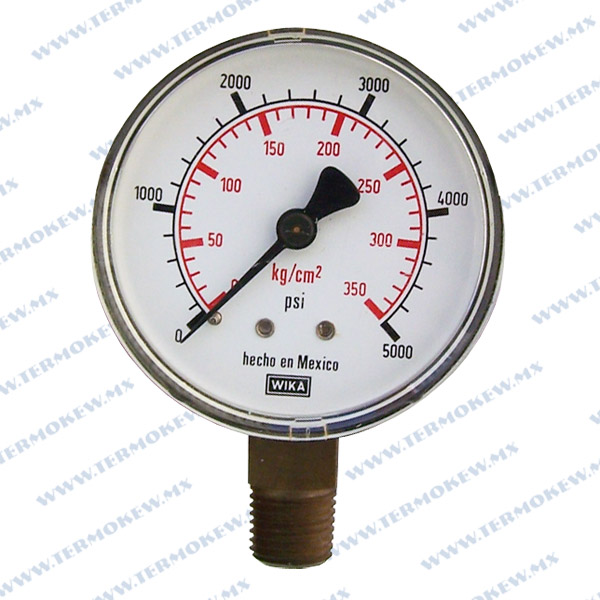
\includegraphics[scale=1.2]{bourdon1.png}
\end{figure}
\subsection{¿Cómo funciona un manómetro de Bourdon?}
l manómetro de Bourdon se basa en el funcionamiento del tubo de Bourdon. Este es un mecanismo que consta de un tubo de forma semicircular donde uno de sus extremos está cerrado, mientras que el otro se encuentra conectado a la fuente de presión.\\
Cuando la presión es aplicada por la parte del tubo abierta, este tiende a enderezarse. Este movimiento es transferido a una aguja que se moverá en forma proporcional a la presión dentro del tubo. Se resalta que la aguja se va a situar delante de una plantilla con las indicaciones del valor de la presión según se relacione con la posición que tenga la aguja.
\subsection{¿Para qué sirve un manómetro de Bourdon?}
El manómetro de Bourdon sirve del mismo modo que los demás manómetros, aunque este es una versión primitiva, para medir la presión de un lugar en particular. En ese sentido, se encarga de medir la presión manométrica, la cual se comprende como la presión total que un gas tiene menos la presión atmosférica, así que la presión atmosférica es despreciada.\\
Se recuerda que los manómetros son muy usados en sitios en los que se necesita medir la presión, pero sin el efecto que la presión atmosférica puede ocasionar, como por ejemplo ocurre con la presión de un gas en un tubo.
\subsection{Partes de un manómetro de Bourdon}
\begin{enumerate}
\item Una aguja.
\item Muelle Bourdon.
\item Una terminal.
\item Un tirante.
\item Un segmento dentado.
\item El movimiento.
\item Un portamuelles.
\end{enumerate}
\begin{figure}[H]
\centering
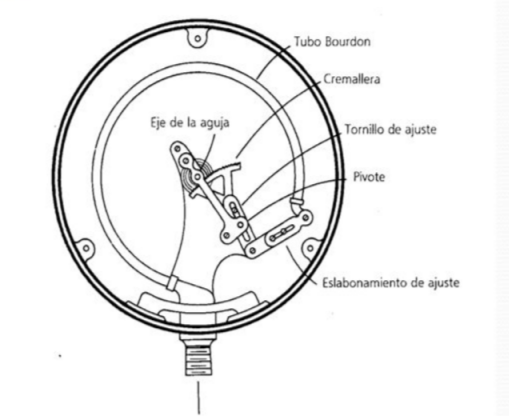
\includegraphics[scale=0.55]{bourdon2.png}
\end{figure}
\section{Calibrador de peso muerto}
\begin{figure}[H]
\centering
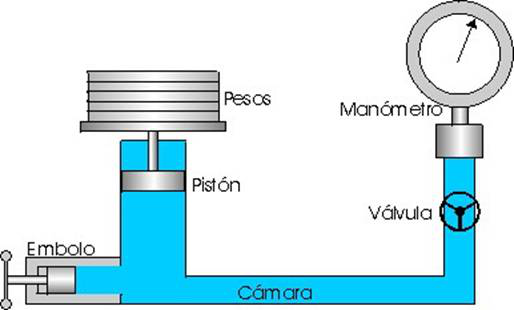
\includegraphics[scale=0.7]{muerto1.png}
\end{figure}
Los medidores de peso muerto son usados para la calibración precisa de manómetros, transductores de presión, etc. El equipo es portátil, de manera que es posible usarlo tanto en demostraciones en el aula, como de calibrador maestro en el laboratorio. El equipo consiste en un sistema de vasos comunicantes que trabaja con aceite bajo el principio de Pascal. Sus partes principales son:
\begin{itemize}
\item Un émbolo
\item Émbolo tornillo
\item Un pistón
\item Un sistema de cañerías
\item Pesas de diferentes medidas
\end{itemize}
Las pesas se colocan en el cilindro hidráulico y girando la válvula principal se regula de tal forma que la cabeza del tornillo quede alineada con la referencia. Si al agregar una pesa el manómetro también aumenta en esa cantidad, entonces se puede decir que está bien calibrado. Ojo, previamente se debe verificar que no haya aire en el sistema de cañerías. Este procedimiento de adición de medición se realiza nuevamente, pero esta vez sustrayendo pesos.\\
Las normas usadas son la Norma NMP 017 de metrología peruana y la norma alemana DNI 1600, DNI 16002, DNI 16003.
\begin{figure}[H]
\centering
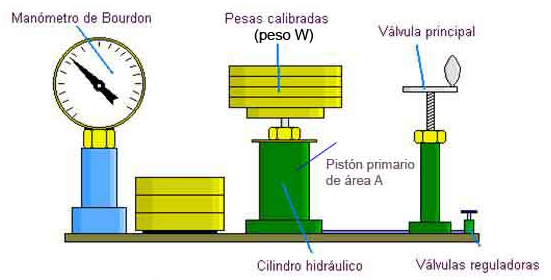
\includegraphics[scale=0.8]{muerto2.png}
\end{figure}
\chapter{Procedimiento}
\begin{enumerate}
\item Desmontamos el equipo, retirando la caja superior desajustando las perillas.
\begin{figure}[H]
\centering
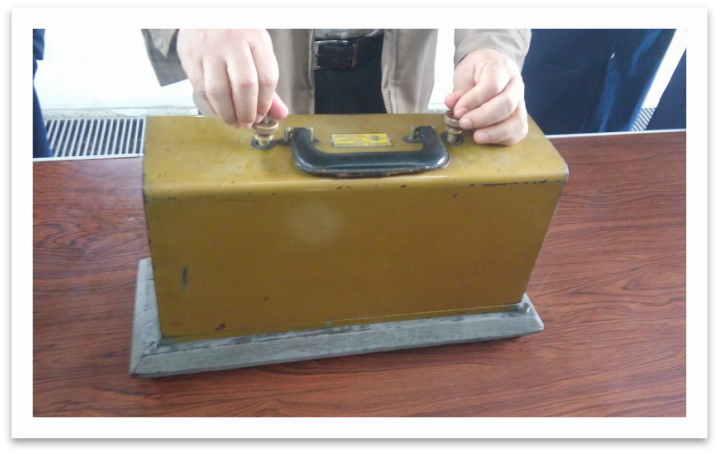
\includegraphics[scale=0.45]{proc1.png}
\end{figure}
\item Procedemos a verificar que el plano de trabajo este nivelado, para esto debemos lograr colocar la burbuja del indicador exactamente en el centro de las marcas.
\begin{figure}[H]
\centering
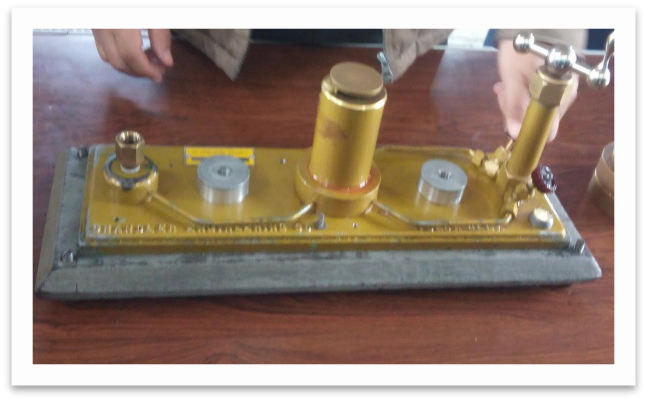
\includegraphics[scale=0.45]{proc2.png}
\end{figure}
\item Retiramos las pesas, verificamos que las válvulas estén completamente cerradas. Abrimos lentamente la válvula reguladora 1 para que el aceite pase al émbolo de tornillo.
\begin{figure}[H]
\centering
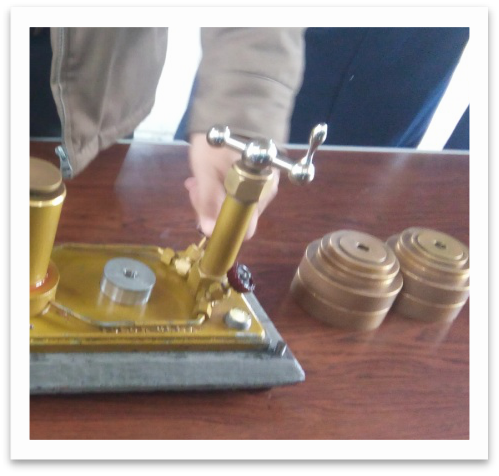
\includegraphics[scale=0.55]{proc3.png}
\end{figure}
\item Cerramos la válvula 1 y se procede a abrir la válvula 2, observamos que el émbolo de tornillo baja empujando el aceite hacia cámara del pistón y hacia la boquilla de salida cuando el aceite llegue a un determinado nivel se procede a colocar el manómetro de Bourdon. Primero ajustamos el manómetro manualmente, luego lo ajustamos completamente con la llave de 1/2 mixta.
\begin{figure}[H]
\centering
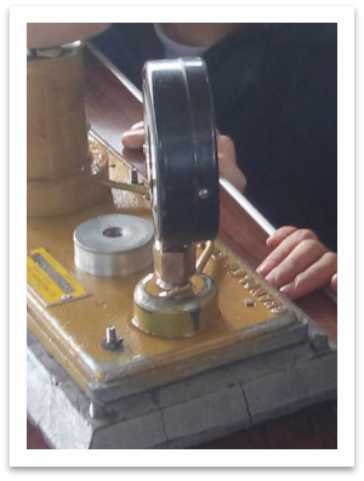
\includegraphics[scale=0.65]{proc4.png}
\end{figure}
\item Giramos la válvula principal hasta alinear el tornillo de referencia y el filo inferior de referencia del pistón. Empezamos con una presión de 5 psi debido al peso del pistón y al área de contacto con el aceite.
\begin{figure}[H]
\centering
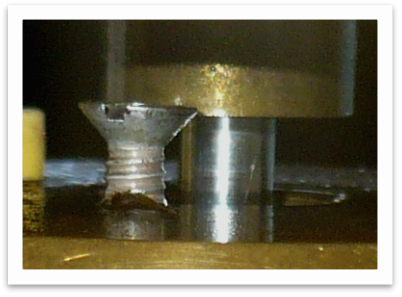
\includegraphics[scale=0.55]{proc5.png}
\end{figure}
\item Repetimos el proceso de medición aumentando la presión en el pistón de 10 en 10 psi por medio de un juego de pesas graduadas, empezando con una presión de 10 psi hasta llegar a 330 psi (ya que a mayores presiones de 330 psi excedemos el rango medible del manómetro de Bourdon). Posteriormente, anotamos la lectura del manómetro para cada presión.
\item Al llegar a los 450 psi de presión se repite el proceso en forma descendente hasta llegar a los 10 psi. 
\item Finalmente, para retirar el manómetro, se abre la válvula reguladora 2 que permite el paso de aceite del pistón al émbolo de tornillo succionando todo el acetite para evitar que se derrame al retirar el manómetro.
\end{enumerate}
\chapter{Cálculos y resultados}
\begin{figure}[H]
\centering
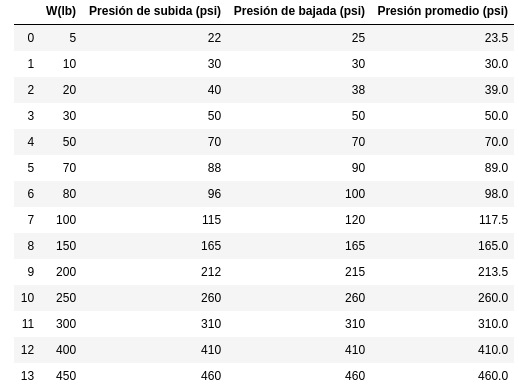
\includegraphics[scale=0.65]{tabla.png}
\end{figure}
La presión medida por el manómetro de bourdon será el promedio obtenido entre los datos de subida con los de bajada.
$$
P_{\mathrm{medida}} = \frac{P_{\mathrm{subida}} + P_{\mathrm{bajada}}}{2}
$$
Se calcula la presión real teniendo en cuenta que el diámetro del pistón es de 1 in.
$$
P_{\mathrm{real}} = \frac{W_{\mathrm{adicionado}}}{\pi/4}
$$
Ya que se tiene un valor real y un valor experimental, aplicamos la formula de \%E mas simple, y que para nuestro caso es más fácil de aplicar.
$$
\% E = \left\vert \frac{P_{\mathrm{real}} - P_{\mathrm{medida}}}{P_{\mathrm{real}}} \right\vert \cdot 100\%
$$
\begin{figure}[H]
\centering
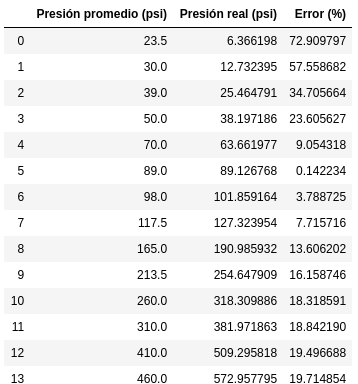
\includegraphics[scale=0.65]{tabla2.png}
\end{figure}
Con dichos resultados se procede a realizar las gráficas correspondientes.
\begin{figure}[H]
\centering
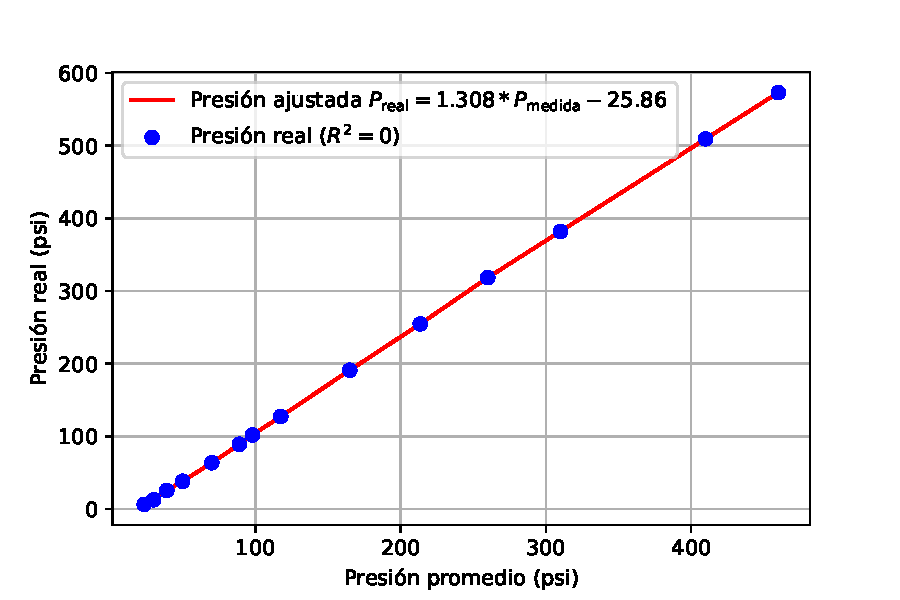
\includegraphics[scale=0.9]{presiones.pdf}
\end{figure}
\chapter{Conclusiones}
\begin{enumerate}
\item Se concluye que el error fluctúa más mientras mayor sea presión, de acuerdo con nuestros datos experimentales.
\item Es de utilidad tener el valor del coeficiente de descarga para estimar el caudal que se obtendrá al usar cualquier dispositivo que pueda afectar el caudal.
\item Al someter a una masa mínima se muestra un porcentaje de error alto, ello es debido a que el circuito muestra obturación; es decir el flujo se limita debido a que sustancias ajenas se adhieren al conducto del fluido
\end{enumerate}
\chapter*{Anexos}
\begin{figure}[H]
\centering
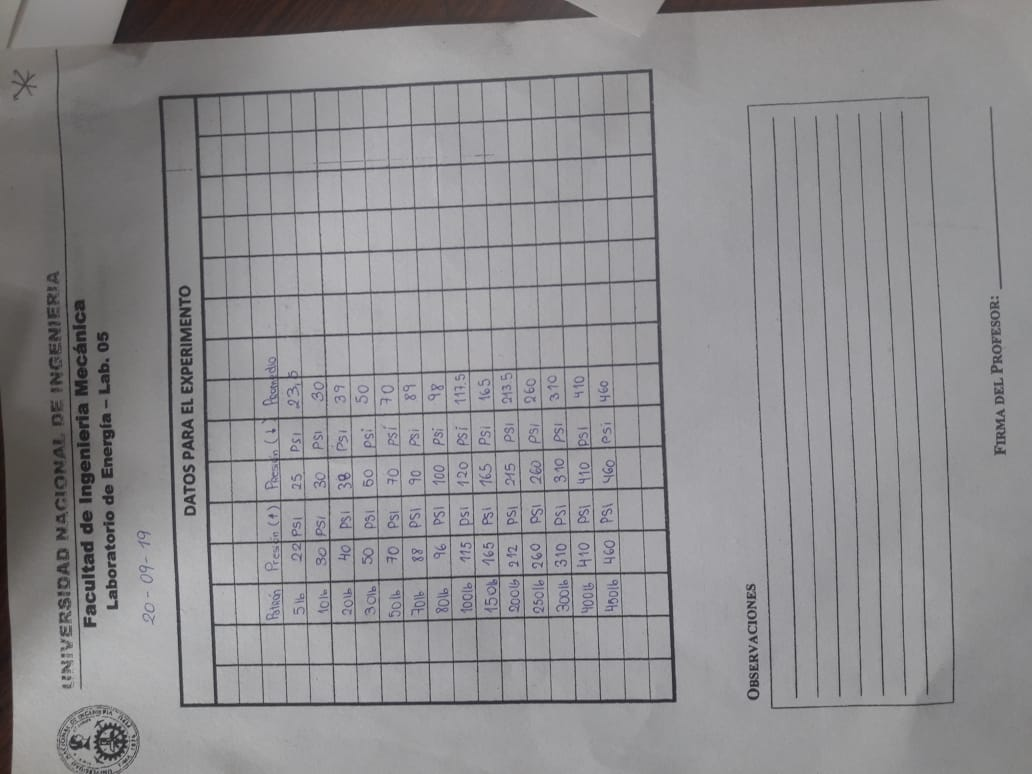
\includegraphics[angle=-90,scale=0.5]{datos.jpeg}
\end{figure}
\begin{thebibliography}{99}  %%%este es un contador para el número de bibliografías utilizados.
\addcontentsline{toc}{chapter}{Bibliograf\'{\i}a} %%% Para introducir la bibliografía en el índice.
%\bibitem{Rahman}{Rahman,Aminur y Doe, Hidekazu; ``Ion transfer of tetraalkylammonium cations at an interface between 
%frozen aqueous solution and 1,2-dichloroethane".{\em{Journal of Electroanalytical Chemistry}} {\bfseries 424},159,(1997).}
\bibitem{Gro}{Chow, V.``Open Channel Hydraulics''.{\em{McGraw-Hill}}}
\bibitem{Gro}{Domínguez, F.``Hidráulica''.}
\bibitem{Ding}{Guevara, Robert (2009).``Manual de prácticas de laboratorio de energía II''.}
\bibitem{AL}{Mott, R. ``Mecánica de fluidos''.\em{Prentice-Hall}}
%\bibitem{AL}{Alonso, Jose M. ``Técnicas de mecanizado 1". {\em{Paraninfo}} {\bfseries España-Madrid}, 6-20, (2001).}
%\bibitem{Samec2}{Samec Z., Lhotsky A., Jänchenová H., y Marecek, V. ``Interfacial tension and impedance measurements
%of interfaces between two inmiscible electrolyte solutions". {\em{Journal of Electroanalytical Chemistry}} {\bfseries
%43}, 47, (2000).}
%\bibitem{Day}{Day R.A. y Underwood A.L. {\textit{Química Analítica Cuantitativa}},5ºed. Prentice-Hall, México, 1998. 45-48.}
%\bibitem{Keyser}{Farah Abud, Michel. ``Determinación de la vida útil en herramientales de corte endurecido por el proceso de borurización en pasta''. {\em{Instituto tecnológico y de estudios superiores de Monterrey}}}
%\bibitem{Zolotorevski}{Escalona, I. ``Máquinas: herramientas por arranque de viruta.''.{\em{El Cid Editor.}}}
%\bibitem{Lasheras}{Lasheras. ``Tecnología de los Materiales Industriales''.} 
%\bibitem{Dieter}{Dieter. ``Metalurgia mecánica''.}
%\bibitem{Apraiz}{Apraiz, J. ``Tratamiento Térmico de los Aceros''.}
%\bibitem{Smith}{Smith, William F. y Ph.D. Hashemi, Javad ``Ciencia e ingeniería de materiales". {\em{
%Madrid: McGraw-Hill, Interamericana de España.}} 570, (2004).} 
%\bibitem{Callister}{Callister, William D. y Rethwisch, David G. ``Introducción a la ingeniería de los materiales''. %{\em{Barcelona Reverté.}}, 960, (2007).} 
%\bibitem{Askeland}{Askeland, Donald R., Pradeep P. Phulé y Wright, Wendelin J. ``Ciencia e ingeniería de los materiales''.{\em{México, D.F. Internacional Thomson Editores.}} {\textit{$6^{ta}$ edición}}, 1004, (2012).}
%\bibitem{HARDBANDING}{Tabla de conversión de escala de durezas. \begin{verbatim}http://%hardbandingsolutions.com/postle_sp/hardness.php
%\end{verbatim}}
%\bibitem{PR}{Termómetro bimetálico. \begin{verbatim}
%https://www.electrabel.es/el-funcionamiento-de-un-termometro-bimetalico/\end{verbatim}}
%\bibitem{PR}{Termómetro de inmersión total. \begin{verbatim}
%http://www.dilabsa.com/es/cual-es-la-diferencia-entre-los-termometros-
%de-inmersion-total-y-parcial/
%\end{verbatim}}
%\bibitem{PR}{Termómetro de inmersión parcial. \begin{verbatim}
%http://www.metas.com.mx/guiametas/La-Guia-MetAs-08-09-termometros-liquido-
%en-vidrio.pdf
%\end{verbatim}}
%\bibitem{HE}{Fresadora. \begin{verbatim} http://lizdenbow.blogspot.com/
%\end{verbatim}}
%\bibitem{ASTM}{Normas ASTM.}
%\bibitem{NTP}{Normas NTP.}
\end{thebibliography}
\end{document}